%% Chapter 4 : Wind Energy Estimation

\section{Kinetic Energy of Air:}
\
\
\
\
The wind turbine converts kinetic energy of air into electrical energy. The kinetic energy possessed by the air is due to the flow of winds. The eq (\ref{W1}) gives the kinetic energy of the air

\begin{equation}
\label{W1}
\text{K.E.(Joules)}=\frac{1}{2}mV^2
\end{equation}\\
where,\\
$ m $ = Mass of Air $ (kg) $\\
$ V $ = Velocity of air $ (m/s) $\\


\section{Power in Wind:}
\
\
\
\
The flow of the mass of air passing through the cross-section of the wind turbine blades is given by the eq (\ref{W2})

\begin{equation}
\label{W2}
\text{mass flowrate} (kg/sec) = mass flow per sec = \rho\times A\times V
\end{equation}

The volumetric flow rate of air is given by the eq (\ref{W3})

\begin{equation}
\label{W3}
\text{volumetric flowrate} (m^3/sec) = A \times V
\end{equation}\\
where,\\
$ \rho $ = Air Density $ (kg/m^{3}) $\\
$ A $ = Swept Area of Rotor $ (m^{2}) $\\

The mass flow rate of air through the cross-section of the wind turbine blades provides for the energy which is converted to electricity.\\


The eq (\ref{W4}) gives us the relationship between power and energy.

\begin{equation}
\label{W4}
\text{Power} = \frac{Energy}{Time}
\end{equation}

The power contained in wind (moving air) is given by eq (\ref{W5}), which is the combination of eq (\ref{W1},\ref{W2},\ref{W3},\ref{W4}).

\begin{equation}
\label{W5}
\text{Power in moving air(Watts)} = \left(\frac{1}{2}\right)\times (mass flow per second)\times V^2 
\end{equation}

The eq (\ref{W6}) combines eq (\ref{W5},\ref{W3}) to give the mechanical power in wind in terms of air density, area and wind velocity; this is a more convenient equation for wind power computations.

\begin{equation}
\label{W6}
\text{Mechanical power in wind(Watts)} = \left(\frac{1}{2}\right) \times (\rho \times A ) \times V^3
\end{equation}

The area in eq (\ref{W6}) in context of wind turbine blades is the rotor-swept area (defined later in the text), but a more general equation of power in wind independent of the area variable is given in the eq (\ref{W7}). It gives the power in wind per meter square of area.

\begin{equation}
\label{W7}
\text{Specific wind power of a site} (W/m^2) = \left(\frac{1}{2}\right) \times \rho \times V^3 
\end{equation}\\



\section{Power Extracted from Wind:}
\
\
\
\
The Fig (\ref{figc5h1}) illustrates the different components of a typical Wind Turbine.

\begin{figure}[H]
\centering
\includegraphics[scale=0.75]{Wind11}
\caption{Wind Turbine [6]}
\label{figc5h1} %% to refer use, \ref{}
\end{figure}

As the wind passes through the cross-section of the wind turbine blades, some portion of its kinetic energy is captured by the wind turbine blades and converted to electricity. In this process the wind loses some of its velocity due to loss of kinetic energy giving us two different wind velocities of upstream (wind velocity in front of the wind turbine) and downstream (wind velocity behind the wind turbine). Hence, the power extracted by the wind turbine from the wind is given by eq (\ref{W8}).

\begin{equation}
\label{W8}
P_0 = \left(\frac{1}{2}\right) \times \text{(mass flow per sec)} \times (V^2 - {V_0}^2)
\end{equation}\\
where,\\
$P_0$ = mechanical power extracted by the rotor (Watts)\\
$ V $ = upstream wind velocity at the entrance of rotor\\
$V_0$ = downstream wind velocity at the exit of rotor \\

The mass of the air passing through the rotor blades is given by the eq (\ref{W9}).

\begin{equation}
\label{W9}
\text{Mass  of air through the rotor blades} (kg/sec) = \rho \times A \times \left(\frac{V + V_0}{2}\right)
\end{equation}

Combining the eq (\ref{W8},\ref{W9}) we get a detailed equation for the mechanical power extracted by the wind turbine rotor from the wind in terms of the eq (ref{W99}).

\begin{equation}
\label{W99}
P_{0}= \frac{1}{2}\left[\rho A \frac{\left(V+V_{0} \right)}{2} \right]\left(V^{2}-V_{0}^{2} \right)
\end{equation}

On further rearranging the eq (\ref{W99}) we get the eq (\ref{W88}).

\begin{equation}
\label{W88}
P_{0} =\frac{1}{2} \rho A V^(3) \frac{\left(1 + \frac{V_0}{V}\right)\times \left[1 - \left(\frac{V_0}{V}\right)^2\right]}{2}
\end{equation}\\

Now the power extracted by the wind turbine rotor blades is expressed as a fraction of upstream wind power in eq (\ref{W10}).

\begin{equation}
\label{W10}
P_0 = \left(\frac{1}{2}\right) \times \rho \times A \times V^3 \times C_p
\end{equation}
where,\\
$C_P$ = Wind Turbine Power Co-efficient\\

The wind Turbine Power Co-efficient is an important variable which depends on the mechanical design of the rotor blades and is given by the eq (\ref{W11}).

\begin{equation}
\label{W11}
C_p = \frac{\left(1 + \frac{V_0}{V}\right)\times \left[1 - \left(\frac{V_0}{V}\right)^2\right]}{2}
\end{equation}

Maximum power extracted from the wind:

\begin{equation}
\label{W12}
P_{max} = \left(\frac{1}{2}\right) \times \rho \times A \times V^3 \times 0.59
\end{equation}\\

Theoretical max. value of $C_p = 0.59$ is called the Betz Limit.

If $C_p = 0.5$, maximum output power of the wind turbine is given by the eq (\ref{W13}).

\begin{equation}
\label{W13}
\text{$P_{max} (Watts/m^2)$}= \left(\frac{1}{4}\right) \times \rho \times V^3 
\end{equation}\\


\section{Effect of Rotor-Swept Area on Wind Power}
\
\
\
\
The rotor-swept area is the cross-sectional area covered by the wind turbine rotor blades. For a horizontal axis wind turbine the rotor-swept area demarcates a circle, and is given by the eq (\ref{W14}).
	
\begin{equation}
\label{W14}
	\text{Rotor swept area}(m^2) = A_H = \left(\frac{\Pi}{4}\right) \times D^2
\end{equation}

From eq (\ref{W10}) we observe that the amount of power extracted by the wind turbine rotor from the wind is directly proportional to the rotor-swept area. Hence, to increase power extraction capacity of a wind turbine the lengths of its rotor blades can be increased.

\section{Effect of Air Density on Wind Power}
\
\
\
\
From eq (\ref{W10}) we can see that the power extracted by a wind turbine is directly proportional to the air density. Hence, denser the air more will be the power extracted from the wind.\\

However, the density of air depends on the on the pressure and temperature of the location as given by the ideal gas law in eq (\ref{W16}).

\begin{equation}
\label{W16}
\rho = \frac{P}{R \times T}
\end{equation}\\
where,\\
$ P $ = Air pressure $ (atm) $\\
$ T $ = Temperature $ (K) $\\
$ R $ = Gas constant $ 8.205745 \time 10^{-5} m^{3} atm K^{-1} mol^(-1) $\\

The air density at sea-level at $1$ atm  $15 \deg$Celsius is $1.2250 kg/m^3$. Using this as a reference $\rho$ is corrected, for the site specific temperature and pressure.Hence, the density of air now is directly proportional to pressure and inversely proportional to temperature of the location.\\

Temperature and pressure both vary with "altitude". Their combined effect is given by the eq (\ref{W17}), which is valid upto $6000$m or $20000$ft of site elevation above sea-level. This equation is however approximate, and the detailed effect of both temperature and pressure on the air density is given in the subsequent sections of the text.

\begin{equation}
\label{W17}
\rho = \rho_0 \times e^{-{\left(\frac{0.297\times H_m}{3048}\right)}}
\end{equation}\\
where,\\
$ \rho $ = Air Density at new height $(kg/m^3)$ \\ 
$ \rho_{o} $ = Air Density at sea level $(kg/m^3)$ \\
$ H_{m} $ = Altitude of the location $(m)$\\


\subsection{Correction for Pressure:}
\
\
\
\

To correct the air density at a given specific location, we first compute the air pressure at the location using its altitude in the eq (\ref{W19}). this gives us the pressure at the specific location.

\begin{equation}
\label{W19}
P = P_{o} \times e^{(-1.185 \times 10^{-4} \times H)}
\end{equation}\\
where,\\
$ P $ = Pressure at new height $(atm)$ \\ 
$ P_{o} $ = Pressure at sea level $(atm)$ \\
$ H_{m} $ = Altitude of the location $(m)$\\


\subsection{Correction for Temperature}
\
\
\
\
After correcting the air pressure for altitude of the location, we use this pressure in the ideal gas law equation along with the temperature of the specific location as given in eq (\ref{W20}).

\begin{equation}
\label{W20}
\rho = \frac{P \times M.W \times 10^{-3}}{R \times T}\\
\end{equation}\\
where,\\
$ M.W $ = Molecular weight of air $  $\\

The eq (\ref{W20}) computes the air density at the specific location accurately as it takes into account both the correction in pressure and temperature.


\section{Effect of Hub-Height on Wind Power:}
\
\
\
\

The wind shear at a ground level surface causes the wind speed to increase with height in accordance with eq (\ref{W36}).

\begin{equation}
\label{W36}
V_2 = V_1 \times \left(\frac{h_2}{h_1}\right)^\alpha
\end{equation}\\
where,\\
$V_1 = \text{wind speed measured at the reference height} \,h_1$\\
$V_2 = \text{wind speed estimated at height} \,h_2$\\
$\alpha = \text{ground surface friction coefficient}$\\

The Table (\ref{c5Tab1}) gives different values of $\alpha$ for different ground surface roughness class.

\begin{table}[H]
  \centering
  \caption{Ground Surface Friction Co-Efficient Claassification}
    \begin{tabular}{|l|c|}
    \hline
    \textbf{Terrain Characteristics} & \multicolumn{1}{l|}{\textbf{Friction Coefficient (α)}} \bigstrut\\
    \hline
    \textbf{Smooth hard ground, calm water } & 0.1 \bigstrut\\
    \hline
    \textbf{Tall grass on level ground } & 0.15 \bigstrut\\
    \hline
    \textbf{High crops, hedges and shrubs } & 0.2 \bigstrut\\
    \hline
    \textbf{Wooded countryside, many trees } & 0.25 \bigstrut\\
    \hline
    \textbf{Small town with trees and shrubs } & 0.3 \bigstrut\\
    \hline
    \textbf{Large city with tall buildings } & 0.4 \bigstrut\\
    \hline
    \end{tabular}%
  \label{c5Tab1}%
\end{table}%

From the eq (\ref{W36}) we can observe that the velocity of wind increases with height. Moreover, as the power extracted from the wind by the wind turbine is directly proportional to the cube of the wind velocity, increasing the hub height has a huge improvement in the power extraction capacity of a wind turbine.\\
	     
\section{Wake Effect Models:}
\
\
\
\
The wake effect is one of the biggest factors for reduction in power capture capacity of wind turbines in a wind farm. The wake effect has two main impacts on the wind farm; firstly there is reduction of wind speed as we move towards the down stream turbines, sometimes causing the downstream turbines to completely stop this causes a considerable amount of loss in power capturing capacity of the wind farm and secondly the the downstream wind is more turbulent causing structural fatigue and eventually lower lifespan of wind turbines. Modeling of Wake Effect helps in the computation of downstream wind velocity deficit (helps in calculating the reduced power capture) and the turbulence patterns so that the wind turbines in a wind farm are arranged spatially to optimize the the power capture. The Fig (\ref{figc5h10}) shows a wake effect simulation in a wind farm.

\begin{figure}[H]
\centering
\includegraphics[scale=0.5]{WakeEffect1}
\caption{Wake effect Simulation}
\label{figc5h10} %% to refer use, \ref{}
\end{figure}

\subsection{Jensen's Model:}
\
\
\
\

The analytical wake model developed by Jensen is simple and requires less inputs as compared other complex wake models. It is used in mostly is optimizing position of the wind turbines within a wind farm. It is based on the global momentum conservation and on the assumption that the wake has a linearly expanding diameter.\\

The Fig (\ref{figc5h11}) illustrates the principle of Jensen's wake model.

\begin{figure}[H]
\centering
\includegraphics[scale=0.5]{WakeEffect2}
\caption{Jensen - Wake Model Principle [56]}
\label{figc5h11} %% to refer use, \ref{}
\end{figure}

The eq (\ref(W44),\ref(W45),\ref(W47),\ref(W48)) describe the Jensen wake model.

\begin{equation}
\label{W44}
	D_{wake} = D(1 + 2ks)\\
\end{equation}\\
    
\begin{equation}
\label{W45}
    u_{def} = U_{\infty}\left[\frac{1-\sqrt{1-C_T}}{(1 + 2ks)^2}\right]\\
\end{equation}\\ 
    
\begin{equation}
\label{W46}
     u = U_{\infty}\left[1 - \frac{1-\sqrt{1-C_T}}{(1 + 2ks)^2}\right]\\
\end{equation}\\
    
\begin{equation}
\label{W47}
     s = x/D\\
\end{equation}\\
    where,\\
    $ D_{wake} $ = Wake Diameter $ (m) $ \\
    $ D $ = Rotor Diameter $ (m) $ \\
    $ k $ = Wake Decay Constant (onshore=0.075 and offshore=0.05) \\
    $ s $ = Normalized downstream distance from turbine $ (m) $ \\
    $ x $ = Axial Distance between Turbines $ (m) $ \\    
    $ u_{def} $ = Velocity deficit in fully developed Wake $ (m/s) $ \\
    $ U_{\infty} $ = Wind Speed $ (m/s) $ \\
    $ C_{T} $ = Induction Factor of Turbine \\
    $ u $ = Wind Speed after Wake effect $ (m/s) $ \\
    
       	 	     
\subsection{Frandsen's Model:}
\
\
\
\
The analytical wake model developed by Frandsen has been adopted in the Storpark Analytical Model (SAM). This model predicts the wind speed deficit in large offshore wind farms using a rectangular site area and straight rows of wind turbines with equidistant spacing between the wind turbines and rows. This model is more accurate than the Jensen model, but requires more input variables.\\

The eq (\ref(W48),\ref(W49),\ref(W50),\ref(W51)) describe the Frandsen wake model.

\begin{equation}
\label{W48}
	D_{wake} = D(\beta ^{(k/2)} + \alpha s)^{\frac{1}{k}}\\
\end{equation}\\
	
\begin{equation}
\label{W49}
	\beta = \frac{1 + \sqrt{1-C_T}}{2 \sqrt{1-C_T}}\\
\end{equation}\\
	
\begin{equation}
\label{W50}
	u_{def} = \frac{U_{\infty}}{2} \left(1 \pm \sqrt{1 - 2 \frac{A}{A_{wake}} C_T}\right)\\
\end{equation}\\	
    
\begin{equation}
\label{W51}
     s = x/D\\
\end{equation}\\
    where,\\
    $ D_{wake} $ = Wake Diameter $ (m) $ \\
    $ D $ = Rotor Diameter $ (m) $ \\
    $ k $ = Wake Decay Constant $ k=2 \text{, for Schlichting solution to the wake expansion; } k=3 \text{, for square root shape chosen } $ \\
    $ \alpha $ = Initial Wake expansion \\
    $ s $ = Normalized downstream distance from turbine $ (m) $ \\
    $ x $ = Axial Distance between Turbines $ (m) $ \\    
    $ u_{def} $ = Velocity deficit in fully developed Wake $ (m/s) $ \\
    $ U_{\infty} $ = Wind Speed $ (m/s) $ \\
    $ C_{T} $ = Induction Factor of Turbine \\
    $ A $ = Swept area of rotor $ (m^{2}) $ \\     
    $ A_{wake} $ = Swept area of Wake $ (m^{2}) $ \\
    
\newpage    
    
\section{Concept of TSR:}
\
\
\
\
Tip Speed Ratio (TSR) is defined as the ratio of the angular speed of the wind turbine rotor blade to the wind velocity, it is given by the eq (\ref{W38}).

\begin{equation}
\label{W38}
TSR = \frac{\text{Linear speed of the blade's outermost tip}}{\text{Free upstream wind velocity}}
\end{equation}\\

The TSR in terms of rotor radius and angular speed in rads/s is given by the eq (\ref{W39}).

\begin{equation}
\label{W39}
TSR = \frac{\omega \times R}{V}
\end{equation}\\
where,\\
$ R $ = rotor radius $ (m) $\\
$\omega$ = angular speed of the rotor $(rads/s)$\\

The TSR is an important quantity in determining the amount of power extracted from wind by the wind turbine, as the Wind Turbine Power Co-efficient $(C_{P})$ is a function of the TSR. The relationship between TSR and $C_{P}$ is dealt with in detail in the next section.\\  


\subsection{Power Coefficient Analysis:}
\
\
\
\
The power extracted from the wind by the wind turbine is directly proportional to the the Wind Turbine Power Co-efficient $(C_{P})$ as seen in the eq (\ref{W10}). $C_{P}$ is experimentally measured by the Wind Turbine Manufactures and its graph is provided in the data-sheet.\\
 
$C_{P}$ describes the aerodynamic behaviour of the wind turbine rotor blades. It is a highly non-linear function of TSR and the blade pitch angle $(\theta)$. For a given $\theta$ the $C_{P}$ is plotted for a range of TSR values. The relationship between $C_{P}$, TSR and $\theta$ differs from turbine to turbine; however, its knowledge helps in designing maximum power tracking controllers which try to maintain $C_{P}$ at its maximum value under the given wind speed condition by adjusting the blade pitch angle (Pitch Control) and/or the gear ratio (Speed Control).\\

The eq (\ref{W41},\ref{W42}) gives a detailed analytical model for the relationship between $C_{P}$, TSR and $\theta$, it is developed by (Anderson & Bose, 1983).

\begin{equation}
\label{W41}
C_p(\lambda , \theta) = C_1\times(C_2  \frac{1}{\beta} - C_3 \beta \theta - C_4 \theta ^x - C_5)e^{-C_6 \frac{1}{\beta}}\\
\end{equation}\\

\begin{equation}
\label{W42}
\frac{1}{\beta} = \frac{1}{\lambda + 0.08\theta} - \frac{0.035}{1 + \theta ^3}\\
\end{equation}\\
where,\\
$ C_{P} $ = Wind Turbine Power Coefficient \\
$ C_{1},C_{2},C_{3},C_{4},C_{5},C_{6} \text{ and }x_ $ = Turbine rotor design dependent constants \\
$ \lambda $ = Tip speed ratio \\

The eq (\ref{W43}) describes another simpler analytical model for C_{P}, which does not take into account physical design differences between the wind turbine rotor blades; it is also developed by (Anderson & Bose, 1983).

\begin{equation}
\label{W43}
	C_p = \frac{1}{2}(\lambda - 0.022\theta ^2 - 5.6)e^{-0.17\lambda}\\
\end{equation}\\	
where,\\ 	
$\lambda = \frac{V_w \text{ (mph) }}{\omega _{b}  (rads_-1) }$\\
where,\\
$ \lambda $ = Tip Speed Ratio \\
$ V_w $ = Wind speed $ (mph) $  \\
$ \omega_b $ = Angular speed of turbine rotor $ (rads/s) $ \\      
    
\section{Weibull Wind Speed Distribution:}
\
\
\
\
The variation in wind speed distribution is best described by the Weibull probability distribution function 'h' with two parameters:

\begin{enumerate}
\item \blindtext The shape parameter 'k'
\item \blindtext The scale parameter 'c'
\end{enumerate}


The probability of wind speed being $\upsilon$ during any time interval is given by eq (\ref{W21})

\begin{equation}
\label{W21}
h(\upsilon) = \left(\frac{k}{c}\right) \times \left(\frac{\upsilon}{c}\right)^{k-1} \times \exp{\left(\frac{\upsilon}{c}\right)}^k \text{, for $0< \upsilon < \infty$}
\end{equation}\\

The eq (\ref{W21}) tells us the probability of occurrence of a particular wind speed. As it is a probability distribution, hence its summation from infinity to infinity is 1. Therefore, we can multiply it with time parameter to get probability of wind speed in terms of hours in a year (if multiplied by 8760) or any other time parameter which fits best for the wind speed being described by the probability distribution.\\

Weibull probability distribution changes its shape according to the shape parameter $k$ as follows:

\begin{enumerate}
\item \blindtext 	$k=1$ makes it the exponential distribution, \,$h = \lambda \times e^{-(\lambda\upsilon)},\, where \, \lambda = \frac{1}			{c}$
\item \blindtext $k=2$ makes it the Rayleigh distribution, \,$h = 2 \times \lambda^2 \times \upsilon \times e^{-(\lambda\upsilon)^2}$
\item \blindtext $k>3$ makes it approach a normal bell-shaped distribution
\end{enumerate}

The eq (\ref{W25}) gives the relationship between the shape parameter (k), scale parameter (c) and the mean wind speed for a give period of time for which the wind data was gathered. Knowing $V_{mean}$ and adjusting the shape parameter (k) so as to come close to the actual wind speed distribution the scale parameter (c) can be computed.

\begin{equation}
\label{W25}
V_{mean} = c \times \sqrt{\left(1 + \frac{1}{k}\right)}
\end{equation}\\


Root mean cube wind speed is defined in similar manner as $V_(rms)$ in AC electrical circuits, it is given by eq (\ref{W28}).

\begin{equation}
\label{W28}
	V_(rmc) = 3 \times \sqrt{\frac{1}{8760}\int\limits_0^\infty h\upsilon^3 \, d\upsilon}
\end{equation}\\

Using $V_{rmc}$ the 'annual average power generation' can be computed as given in eq (\ref{W29}).

\begin{equation}
\label{W29}
	P_{rmc} = \frac{1}{4}\times \rho \times {V_{rmc}}^3
\end{equation}\\

Furthermore, using eq (\ref{W30}) we can compute the average annual energy production of the specific site.
	
\begin{equation}
\label{W30}
	\text{Average annual energy production of the site} = P_{rmc} \times \text{total number of hours per year}
\end{equation}\\

So, using the concepts of Weibull Distribution and Root Mean Cube Wind Speed, we can estimate the potential of a site for setting up a wind farm with minimum amount of data (just annual mean wind speed can suffice for performing the analysis).\\

\newpage 
		
\section{Power Flow through Wind Turbine Grid Connected System}
\
\
\
\
The Fig (\ref{Windloss}) illustrates the power flow through a Wind Turbine grid connected system and the various losses incurred in the this system.

\begin{figure}[H]
\centering
\includegraphics[scale=0.75]{WindLoss1}
\caption{Flow Diagram - Power Flow and Power Losses in a Wind Turbine Grid Connected System}
\label{WindLoss} %% to refer use, \ref{}
\end{figure}

\subsection{Wind Speed Correction}
\
\
\
\
The wind speed measured in a Wind Turbine Power Plant by a weather station at ground level. In order to know the exact wind speed at the height of the wind turbine rotors, correction has to be implemented as directed by the eq (\ref{}).

Moreover, wake effect has to be taken into account to incorporate the downstream wind velocity deficit as explained in the section (5.7), either using Jensen or Frandsen wake effect models.

\subsection{Power Curve Correction}
\
\
\
\ 
As discussed in the section (5.5), the air density has a direct proportion to the power extracted by the wind turbine from the wind. The Power vs Wind Speed curves provided by the manufacturers are experimentally measured at sea level at a controlled temperature of $15^{\circ}C$. However the the altitude and the temperature at the specific wind farm location is different, hence power curve correction based on the air density correction has to performed for more accurate power estimation from the wind turbines.

\subsection{Ohmic and Transformer Losses}
\
\
\
\	
AC cabling is done to connect wind turbines to the transformer. All these cables add to the resistance of the Wind Turbine system causing huge ohmic losses. Hence, in order to reduce these ohmic losses, the length of the cabling should be minimum and the cable material should be of low resistivity.\\

Transformers are another indispensible part of the grid connected Wind Turbine systems. They step-up the voltage of the Wind Turbine system output, so that the power can be transferred to the transmission lines operating at higher voltages. But, transformers consist of copper coils which result in resistive losses, and iron cores which cause iron losses. Hence, the power output to the grid from the the PV system is reduced.\\  

\newpage
    
\section{MATLAB Model Algorithm}   

The Fig (\ref{figc5h4} ) depicts an simplified flowchart of the algorithm which is developed for the creation of the Wind Energy Estimation Application. 	      	 	
  
\begin{figure}[H]
\centering
\includegraphics[scale=0.5]{WindScheme}
\caption{Wind Turbine Energy Estimation Schematic}
\label{figc5h4} %% to refer use, \ref{}
\end{figure}

Based on the theory discussed in previous sections of this chapter and the algorithm developed as illustrated in Fig (\ref{WindLoss1},\ref{figc5h4}); a GUI based application for energy estimation of grid connected wind turbine power plants is developed in MATLAB, the results of which are presented in the next section and the application GUIs can be found in the Appendix.

\newpage

\section{Results}
\
\
\
\
The Wind Energy Estimation App has been tested with a hypothetical wind turbine power plant, and the Weibull Distribution sub-module has been tested with random site information. The results obtained are doumented in the following sections.

\subsection{Wind Turbine Power Plant Site Potential Estimation using Weibull Distribution App}
\
\
\
\
The Fig (\ref{WinResImg1}) shows the site potential estimation performed by the Weibull Distribution sub-module for monthly data.

\begin{figure}[H]
\centering
\includegraphics[scale=0.5]{Weibull_Monthly}
\caption{Weibull Distribution-Monthly Simulation }
\label{WinResImg1} %% to refer use, \ref{}
\end{figure}

The Fig (\ref{WinResImg2}) shows the site potential estimation performed by the Weibull Distribution sub-module for yearly data.

\begin{figure}[H]
\centering
\includegraphics[scale=0.5]{Weibull_Yearly}
\caption{ Weibull Distribution-Yearly Simulation }
\label{WinResImg2} %% to refer use, \ref{}
\end{figure}

\subsection{Cp Curve Generator App}
\
\
\
\
The Table (\ref{CpCurveTab1}) gives the rotor information used to generate C_{P} curves using equation (\ref{W41}).

\begin{table}[htbp]
  \centering
  \caption{Cp Curve Generator App - Equation 1 Simulation Parameters}
    \begin{tabular}{|l|l|}
    \hline
    \multicolumn{2}{|c|}{\textbf{Cp Curve Equation 1}} \bigstrut\\
    \hline
    \multicolumn{1}{|c|}{\textbf{Parameters }} & \multicolumn{1}{c|}{\textbf{Value}} \bigstrut\\
    \hline
    \multicolumn{1}{|c|}{Number of Rotor Types} & 3 \bigstrut\\
    \hline
    c1 & 0.5,0.7,0.3 \bigstrut\\
    \hline
    c2 & 116,150,85 \bigstrut\\
    \hline
    c3 & 0.4,0.6,0.2 \bigstrut\\
    \hline
    c4 & 0,0,0 \bigstrut\\
    \hline
    c5 & 5,10,3 \bigstrut\\
    \hline
    c6 & 21,31,11 \bigstrut\\
    \hline
    x  & 0,0,0 \bigstrut\\
    \hline
    Theta & 1,2,3,4 \bigstrut\\
    \hline
    \end{tabular}%
  \label{CpCurveTab1}%
\end{table}%

The Fig (\ref{WinResImg3},\ref{WinResImg4},\ref{WinResImg5}) shows the C_{P} curve graphs obtained from the Cp Curve Generator App for different values of the blade pitch angles.

\begin{figure}[H]
\centering
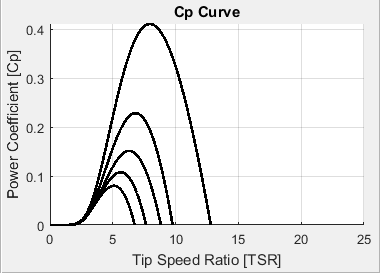
\includegraphics[scale=0.5]{CpCurve_Eq1_1}
\caption{CpCurve Generator App-Equation 1 Rotor 1 Simulation}
\label{WinResImg3} %% to refer use, \ref{}
\end{figure}

\begin{figure}[H]
\centering
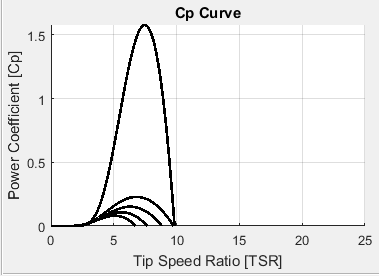
\includegraphics[scale=0.5]{CpCurve_Eq1_2}
\caption{CpCurve Generator App-Equation 1 Rotor 2 Simulation}
\label{WinResImg4} %% to refer use, \ref{}
\end{figure}
\begin{figure}[H]

\centering
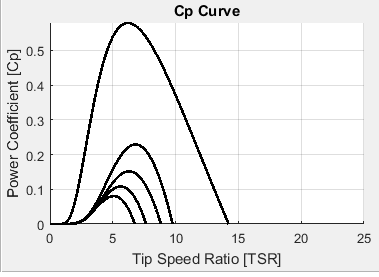
\includegraphics[scale=0.5]{CpCurve_Eq1_3}
\caption{CpCurve Generator App-Equation 1 Rotor 3 Simulation}
\label{WinResImg5} %% to refer use, \ref{}
\end{figure}

The Table (\ref{CpCurveTab2}) gives the rotor information used to generate C_{P} curves using equation (\ref{W43}).

\begin{table}[htbp]
  \centering
  \caption{Cp Curve Generator App - Equation 2 Simulation Parameters}
    \begin{tabular}{|l|l|}
    \hline
    \multicolumn{2}{|c|}{\textbf{Cp Curve Equation 2}} \bigstrut\\
    \hline
    \multicolumn{1}{|c|}{\textbf{Parameters }} & \multicolumn{1}{c|}{\textbf{Value}} \bigstrut\\
    \hline
    Number of Rotor Types &  \bigstrut\\
    \hline
    c1 & 0.5 \bigstrut\\
    \hline
    c2 & 116 \bigstrut\\
    \hline
    c3 & 0.4 \bigstrut\\
    \hline
    c4 & 0 \bigstrut\\
    \hline
    c5 & 5 \bigstrut\\
    \hline
    c6 & 21 \bigstrut\\
    \hline
    x  & 0 \bigstrut\\
    \hline
    Theta & 0,5,10,15,20 \bigstrut\\
    \hline
    \end{tabular}%
  \label{CpCurveTab2}%
\end{table}%

The Fig (\ref{WinResImg6}) shows the C_{P} curve graphs obtained from the Cp Curve Generator App for different values of the blade pitch angles.

\begin{figure}[H]
\centering
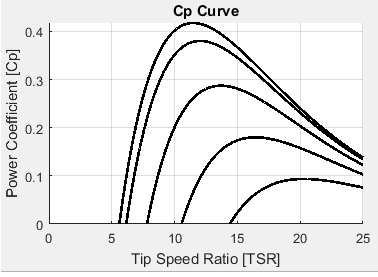
\includegraphics[scale=0.5]{CpCurve_Eq2_1}
\caption{CpCurve Generator App-Equation 2 Simulation }
\label{WinResImg6} %% to refer use, \ref{}
\end{figure}


\subsection{Hypothetical Wind Turbine Plant Information}
\
\
\
\
The Table (\ref{DataTab1}) gives the information of the hypothetical wind power plant, which was fed into the Data Acquisition App and the Wind Energy Estimation App for testing purposes due lack of real WTPP data.

\begin{table}[H]
  \centering
  \captionHypothetical Wind Turbine Power Plant Information Table}
    \begin{tabular}{|l|l|l|l|l|}
    \hline
    \multicolumn{5}{|c|}{\textbf{HYPOTHETICAL WIND TURBINE POWER PLANT}} \bigstrut\\
    \hline
    \multicolumn{5}{|c|}{\textbf{SITE INFORMATION}} \bigstrut\\
    \hline
    \textbf{LATITUDE} & \multicolumn{4}{l|}{23.275} \bigstrut\\
    \hline
    \textbf{LONGITUDE} & \multicolumn{4}{l|}{72.682} \bigstrut\\
    \hline
    \textbf{ALTITUDE (m)} & \multicolumn{4}{l|}{100} \bigstrut\\
    \hline
    \textbf{PLANT CAPACITY (MW)} & \multicolumn{4}{l|}{138} \bigstrut\\
    \hline
    \multicolumn{5}{|c|}{\textbf{WIND TURBINE PLANT INFORMATION}} \bigstrut\\
    \hline
    \textbf{PARAMETERS} & \multicolumn{4}{c|}{\textbf{WIND GENERATOR TYPES}} \bigstrut\\
    \hline
       & \textbf{Type1} & \textbf{Type2} & \textbf{Type3} & \textbf{Type4} \bigstrut\\
    \hline
    \textbf{No. of Sub-Models} & 1  & 2  & 3  & 4 \bigstrut\\
    \hline
    \textbf{No. of Turbines} & 5  & 5,10 & 5,10,15 & 5,10,15,20 \bigstrut\\
    \hline
    \textbf{Cut-In Wind Speed} & 4  & 4,4 & 4,4,4 & 4,4,4,3.5 \bigstrut\\
    \hline
    \textbf{Cut-Out Wind Speed} & 24 & 24,19 & 24,19,25 & 24,19,25,23 \bigstrut\\
    \hline
    \textbf{Rotor Radius} & 38.5 & 38.5,19.5 & 38.5,19.5,35.5 & 38.5,19.5,35.5,38.5 \bigstrut\\
    \hline
    \textbf{Hub-Height} & 80 & 80,55 & 80,55,73 & 80,50,73,80 \bigstrut\\
    \hline
    \end{tabular}%
  \label{DataTab1}%
\end{table}%



\subsection{Wind Turbine Power Curve GUI}
\
\
\
\
The Fig (\ref{WinResImg7},\ref{WinResImg8},\ref{WinResImg9},\ref{WinResImg10}) illustrates the Power (kW) vs Wind Speed (m/s) graphs of the four different wind turbines used in the simulation as observed in the Wind Power Curves sub-module.

\begin{figure}[H]
\centering
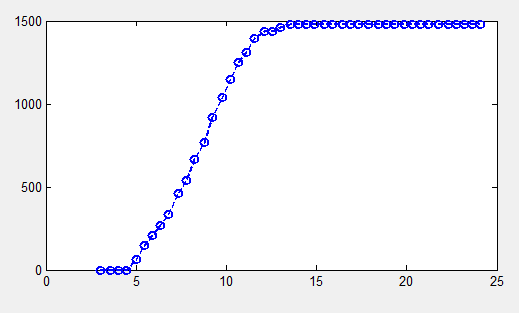
\includegraphics[scale=0.5]{NegMicon}
\caption{Power vs Wind Speed Curve-Neg Micon 1.5MW}
\label{WinResImg7} %% to refer use, \ref{}
\end{figure}

\begin{figure}[H]
\centering
\includegraphics[scale=0.5]{Vestas}
\caption{Power vs Wind Speed Curve-Vestas 0.6MW}
\label{WinResImg8} %% to refer use, \ref{}
\end{figure}

\begin{figure}[H]
\centering
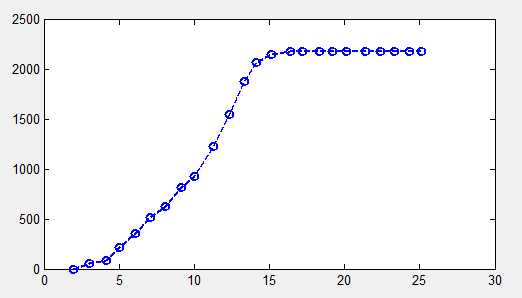
\includegraphics[scale=0.5]{Enercon}
\caption{Power vs Wind Speed Curve-Enercon 2MW }
\label{WinResImg9} %% to refer use, \ref{}
\end{figure}

\begin{figure}[H]
\centering
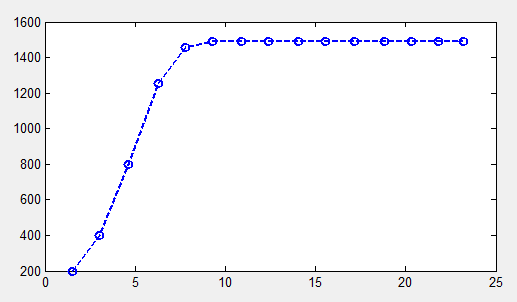
\includegraphics[scale=0.5]{GE}
\caption{Power vs Wind Speed Curve-GE 1.5MW}
\label{WinResImg10} %% to refer use, \ref{}
\end{figure}


\subsection{Wind Energy Estimation App Output}
\
\
\
\
The Fig (\ref{WinResImg11}) shows the monthly energy output to the grid obtained from the four different types of wind turbines present in the type four category of the hypothetical wind power plant as computed in the Wind Energy Estimation App. The wind speed data was randomly generated and the temperature data was taken from Meteonorm, both at the temporal resolution of 60 minutes.

\begin{figure}[H]
\centering
\includegraphics[scale=0.5]{WindGraph1}
\caption{Hypothetical Wind Plant Month Wise Energy Estimation For Different Wind Generator Types}
\label{WinResImg11} %% to refer use, \ref{}
\end{figure}

We can clearly see that the energy output of the Enercon and GE  compared to Neg Micon and Vestas is higher, as the number of these turbines is higher.




